% Options for packages loaded elsewhere
\PassOptionsToPackage{unicode}{hyperref}
\PassOptionsToPackage{hyphens}{url}
%
\documentclass[
]{article}
\usepackage{lmodern}
\usepackage{amssymb,amsmath}
\usepackage{ifxetex,ifluatex}
\ifnum 0\ifxetex 1\fi\ifluatex 1\fi=0 % if pdftex
  \usepackage[T1]{fontenc}
  \usepackage[utf8]{inputenc}
  \usepackage{textcomp} % provide euro and other symbols
\else % if luatex or xetex
  \usepackage{unicode-math}
  \defaultfontfeatures{Scale=MatchLowercase}
  \defaultfontfeatures[\rmfamily]{Ligatures=TeX,Scale=1}
\fi
% Use upquote if available, for straight quotes in verbatim environments
\IfFileExists{upquote.sty}{\usepackage{upquote}}{}
\IfFileExists{microtype.sty}{% use microtype if available
  \usepackage[]{microtype}
  \UseMicrotypeSet[protrusion]{basicmath} % disable protrusion for tt fonts
}{}
\makeatletter
\@ifundefined{KOMAClassName}{% if non-KOMA class
  \IfFileExists{parskip.sty}{%
    \usepackage{parskip}
  }{% else
    \setlength{\parindent}{0pt}
    \setlength{\parskip}{6pt plus 2pt minus 1pt}}
}{% if KOMA class
  \KOMAoptions{parskip=half}}
\makeatother
\usepackage{xcolor}
\IfFileExists{xurl.sty}{\usepackage{xurl}}{} % add URL line breaks if available
\IfFileExists{bookmark.sty}{\usepackage{bookmark}}{\usepackage{hyperref}}
\hypersetup{
  pdftitle={Note on combining p values of GWAS studies from different populations},
  pdfauthor={Ziang Zhang},
  hidelinks,
  pdfcreator={LaTeX via pandoc}}
\urlstyle{same} % disable monospaced font for URLs
\usepackage[margin=1in]{geometry}
\usepackage{color}
\usepackage{fancyvrb}
\newcommand{\VerbBar}{|}
\newcommand{\VERB}{\Verb[commandchars=\\\{\}]}
\DefineVerbatimEnvironment{Highlighting}{Verbatim}{commandchars=\\\{\}}
% Add ',fontsize=\small' for more characters per line
\usepackage{framed}
\definecolor{shadecolor}{RGB}{248,248,248}
\newenvironment{Shaded}{\begin{snugshade}}{\end{snugshade}}
\newcommand{\AlertTok}[1]{\textcolor[rgb]{0.94,0.16,0.16}{#1}}
\newcommand{\AnnotationTok}[1]{\textcolor[rgb]{0.56,0.35,0.01}{\textbf{\textit{#1}}}}
\newcommand{\AttributeTok}[1]{\textcolor[rgb]{0.77,0.63,0.00}{#1}}
\newcommand{\BaseNTok}[1]{\textcolor[rgb]{0.00,0.00,0.81}{#1}}
\newcommand{\BuiltInTok}[1]{#1}
\newcommand{\CharTok}[1]{\textcolor[rgb]{0.31,0.60,0.02}{#1}}
\newcommand{\CommentTok}[1]{\textcolor[rgb]{0.56,0.35,0.01}{\textit{#1}}}
\newcommand{\CommentVarTok}[1]{\textcolor[rgb]{0.56,0.35,0.01}{\textbf{\textit{#1}}}}
\newcommand{\ConstantTok}[1]{\textcolor[rgb]{0.00,0.00,0.00}{#1}}
\newcommand{\ControlFlowTok}[1]{\textcolor[rgb]{0.13,0.29,0.53}{\textbf{#1}}}
\newcommand{\DataTypeTok}[1]{\textcolor[rgb]{0.13,0.29,0.53}{#1}}
\newcommand{\DecValTok}[1]{\textcolor[rgb]{0.00,0.00,0.81}{#1}}
\newcommand{\DocumentationTok}[1]{\textcolor[rgb]{0.56,0.35,0.01}{\textbf{\textit{#1}}}}
\newcommand{\ErrorTok}[1]{\textcolor[rgb]{0.64,0.00,0.00}{\textbf{#1}}}
\newcommand{\ExtensionTok}[1]{#1}
\newcommand{\FloatTok}[1]{\textcolor[rgb]{0.00,0.00,0.81}{#1}}
\newcommand{\FunctionTok}[1]{\textcolor[rgb]{0.00,0.00,0.00}{#1}}
\newcommand{\ImportTok}[1]{#1}
\newcommand{\InformationTok}[1]{\textcolor[rgb]{0.56,0.35,0.01}{\textbf{\textit{#1}}}}
\newcommand{\KeywordTok}[1]{\textcolor[rgb]{0.13,0.29,0.53}{\textbf{#1}}}
\newcommand{\NormalTok}[1]{#1}
\newcommand{\OperatorTok}[1]{\textcolor[rgb]{0.81,0.36,0.00}{\textbf{#1}}}
\newcommand{\OtherTok}[1]{\textcolor[rgb]{0.56,0.35,0.01}{#1}}
\newcommand{\PreprocessorTok}[1]{\textcolor[rgb]{0.56,0.35,0.01}{\textit{#1}}}
\newcommand{\RegionMarkerTok}[1]{#1}
\newcommand{\SpecialCharTok}[1]{\textcolor[rgb]{0.00,0.00,0.00}{#1}}
\newcommand{\SpecialStringTok}[1]{\textcolor[rgb]{0.31,0.60,0.02}{#1}}
\newcommand{\StringTok}[1]{\textcolor[rgb]{0.31,0.60,0.02}{#1}}
\newcommand{\VariableTok}[1]{\textcolor[rgb]{0.00,0.00,0.00}{#1}}
\newcommand{\VerbatimStringTok}[1]{\textcolor[rgb]{0.31,0.60,0.02}{#1}}
\newcommand{\WarningTok}[1]{\textcolor[rgb]{0.56,0.35,0.01}{\textbf{\textit{#1}}}}
\usepackage{graphicx,grffile}
\makeatletter
\def\maxwidth{\ifdim\Gin@nat@width>\linewidth\linewidth\else\Gin@nat@width\fi}
\def\maxheight{\ifdim\Gin@nat@height>\textheight\textheight\else\Gin@nat@height\fi}
\makeatother
% Scale images if necessary, so that they will not overflow the page
% margins by default, and it is still possible to overwrite the defaults
% using explicit options in \includegraphics[width, height, ...]{}
\setkeys{Gin}{width=\maxwidth,height=\maxheight,keepaspectratio}
% Set default figure placement to htbp
\makeatletter
\def\fps@figure{htbp}
\makeatother
\setlength{\emergencystretch}{3em} % prevent overfull lines
\providecommand{\tightlist}{%
  \setlength{\itemsep}{0pt}\setlength{\parskip}{0pt}}
\setcounter{secnumdepth}{5}
\usepackage{amsmath,amsthm, amssymb}
\usepackage{booktabs}
\usepackage{longtable}
\usepackage{array}
\usepackage{multirow}
\usepackage{wrapfig}
\usepackage{float}
\usepackage{colortbl}
\usepackage{pdflscape}
\usepackage{tabu}
\usepackage{threeparttable}
\usepackage{threeparttablex}
\usepackage[normalem]{ulem}
\usepackage{makecell}
\usepackage{xcolor}

\title{\textbf{Note on combining p values of GWAS studies from different
populations}}
\author{Ziang Zhang}
\date{4/17/2021}

\begin{document}
\maketitle

\newcommand{\p}{\text{P}}
\newcommand{\E}{\mathbb{E}}
\newcommand{\Var}{\text{Var}}

\hypertarget{introduction}{%
\section{Introduction:}\label{introduction}}

For most traits,genetic effects from specific SNP only have small effect
sizes(Evangelou and Ioannidis 2013). Therefore, practitioners often
aggregate the GWAS results from different population through different
kinds of meta-analysis methods in order to achieve higher power.
Aggregation through P values is a commonly used example of meta-analysis
method. For example when there are several different datasets,
practitioners sometimes will first carry out a comprehensive study using
one dataset, and only study the SNPs with highest significance levels in
the rest datasets (Begum et al. 2012). Hence, we would like to consider
when such procedure will no longer be valid in this note.

In this note, by examining the power and distribution of P values of
Wald test, we conclude that the same hypothesis test on different
populations can have very different P values under the alternative
hypothesis, hence power, even when there is no heterogeneity on the true
SNP effect and the covariates among the two populations.

In next section, we will give a brief overview of Wald tests for
Generalized Linear Models, and a short explanation of the rationale
behind this phenomenon. Then, we will follow with two simulation studies
to illustrate how this phenomenon occurs for binary trait.

\hypertarget{wald-test-for-generalized-linear-models}{%
\section{Wald test for Generalized Linear
Models:}\label{wald-test-for-generalized-linear-models}}

Assume the generalized linear model (glm) has the following form:
\[\mathbb{E}(Y|X) = \mu = g^{-1}(\beta_0 + \beta_1 X_1 + \beta_2X_2) = g^{-1}(\eta),\]
where \(g(.)\) is a specific link function connecting the linear
predictor \(\eta\) with the mean function of \(Y\). In this case, the
fisher information matrix at \(\beta\) can be written as
\[I_n(\beta) = XW(\beta) X^T,\] where X denotes the design matrix and
\(W(\beta)\) is a diagonal matrix with each diagonal term depending on
the value of \(\beta\) unless \(g\) is identity function. Specifically,
the \(i^{th}\) diagonal term of W can be computed as
\[w_i=(\frac{\partial u_i}{\partial\eta_i})^2/\text{Var}(Y_i|X).\]

If the question of interest is to test the hypothesis \(H_0: \beta_2=0\)
using Wald test, the test statistic can be written as
\[T = I_n^{-1}(\hat{\beta})_{[3,3]}(\hat{\beta_2})^2,\] where
\(I_n^{-1}(\hat{\beta})_{[3,3]}\) denotes the third diagonal term of the
matrix \(I_n^{-1}(\hat{\beta})\) and \(\hat{\beta}\) is the MLE
estimator. Under the null hypothesis, \(T\) asymptotically follows a
Chi-Square distribution with 1 degree of freedom.

Under the alternative hypothesis that
\(\beta_2 = \tilde{\beta}_2 \neq 0\), the non-centrality parameter of
Wald test above can be computed as
\[I_n^{-1}(\tilde{\beta})_{[3,3]}\tilde{\beta}_2^2,\] where
\(\tilde{\beta}\) is the vector of true values for the regression
parameters \(\beta\). Since \(I_n^{-1}(\tilde{\beta})_{[3,3]}\) will not
solely depend on \(\tilde{\beta}_2\) unless \(g\) is identity. Therefore
the power function of this Wald test will not only depend on
\(\tilde{\beta}_2\), but the whole vector \(\tilde{\beta}\).

Define \(d=-\sqrt{I_n^{-1}(\tilde{\beta})_{[3,3]}}\tilde{\beta}_3\), the
theoretical power of this Wald test at \(\tilde{\beta}\) can be computed
as \[1-\Phi(d+z_{a/2})+\Phi(d-z_{a/2}),\] where \(\Phi\) is the CDF of
standard normal and \(z_{a/2}\) is the \(a/2\) quantile of standard
normal.

\hypertarget{simulation-with-random-samples}{%
\section{Simulation with random
samples:}\label{simulation-with-random-samples}}

Consider that two samples of size \(n=1000\) have been collected
independently on two populations (European, Asian), and question of
interest is to study the association between the status of a particular
disease (\(Y:0/1\)) and a particular SNP \(G\) with minor allele
frequency (MAF) \(0.3\) under Hardy Weinberg Equilibrium (HWE), after
controlling the effect of a covariate Z (\(Z\sim N(0,\sigma=3)\)).

Assume that GWAS study has been carried out for each population to test
if the SNP \(G\) is causal for \(Y\), and the p-values are
\(5\times10^{-4}\) for European population and \(5 \times 10^{-8}\) for
Asian population, can we interpret the result as there is likely a
stronger association in Asian population than European population? To
answer this question, we will conduct the following simulation study.

We assume that the models that generate the observations for European
population and for Asian population are the followings:
\[\textbf{Euro}:\text{logit}(\text{P}(Y=1|G,Z)) = -0.5 + 0.8Z + 0.3G,\]
\[\textbf{Asian}: \text{logit}(\text{P}(Y=1|G,Z)) = -0.5 + 0.1Z + 0.3G.\]

In other words, the effect of Z will be different across the two
populations, but the effect of the SNP will be the same. We generated
\(\{G_i\}_n\) and \(\{Z_i\}_n\) independently, and used the same set of
covariates to generate the response variables in each population.

\hypertarget{summary-of-simulated-data-and-p-values}{%
\subsection{Summary of simulated data and P
values:}\label{summary-of-simulated-data-and-p-values}}

In our simulation, the same sets of \(G\) and \(Z\) will be used to
simulate traits in both populations. We simulated \(\{G_i\}\)
independently from \(\{Z_i\}\), and then simulated the disease status
\(Y\) using \(G\) and \(Z\). Recall that \(Z \sim N(0,3)\) and MAF of
\(G\) is 0.3. The summary of our generated data is present at below:

\begin{Shaded}
\begin{Highlighting}[]
\CommentTok{### Simulated the common Z and G}
\KeywordTok{set.seed}\NormalTok{(}\DecValTok{100}\NormalTok{,}\DataTypeTok{sample.kind =} \StringTok{"Rounding"}\NormalTok{)}
\NormalTok{N <-}\StringTok{ }\DecValTok{1000}
\NormalTok{G <-}\StringTok{ }\KeywordTok{sample}\NormalTok{(}\KeywordTok{c}\NormalTok{(}\DecValTok{0}\NormalTok{,}\DecValTok{1}\NormalTok{,}\DecValTok{2}\NormalTok{),}\DataTypeTok{size =}\NormalTok{ N, }\DataTypeTok{replace =}\NormalTok{ T, }\DataTypeTok{prob =} \KeywordTok{c}\NormalTok{(}\FloatTok{0.49}\NormalTok{,}\FloatTok{0.42}\NormalTok{,}\FloatTok{0.09}\NormalTok{))}
\NormalTok{Z <-}\StringTok{ }\KeywordTok{rnorm}\NormalTok{(N,}\DataTypeTok{sd =} \DecValTok{3}\NormalTok{)}


\CommentTok{### Simulate each population's disease status based on Z and G}
\CommentTok{## Eur:}
\NormalTok{beta0 <-}\StringTok{ }\FloatTok{-0.5}
\NormalTok{betaZ <-}\StringTok{ }\FloatTok{0.8}
\NormalTok{betaG <-}\StringTok{ }\FloatTok{0.3}
\NormalTok{ylat_Eur <-}\StringTok{ }\NormalTok{beta0 }\OperatorTok{+}\StringTok{ }\NormalTok{betaG}\OperatorTok{*}\NormalTok{G }\OperatorTok{+}\StringTok{ }\NormalTok{betaZ}\OperatorTok{*}\NormalTok{Z }\OperatorTok{+}\StringTok{ }\KeywordTok{rlogis}\NormalTok{(N)}
\NormalTok{y_Eur <-}\StringTok{ }\KeywordTok{ifelse}\NormalTok{(ylat_Eur }\OperatorTok{>=}\DecValTok{0}\NormalTok{, }\DecValTok{1}\NormalTok{, }\DecValTok{0}\NormalTok{)}

\CommentTok{## Asia:}
\NormalTok{beta0 <-}\StringTok{ }\FloatTok{-0.5}
\NormalTok{betaZ <-}\StringTok{ }\FloatTok{0.1}
\NormalTok{betaG <-}\StringTok{ }\FloatTok{0.3}
\NormalTok{ylat_As <-}\StringTok{ }\NormalTok{beta0 }\OperatorTok{+}\StringTok{ }\NormalTok{betaG}\OperatorTok{*}\NormalTok{G }\OperatorTok{+}\StringTok{ }\NormalTok{betaZ}\OperatorTok{*}\NormalTok{Z }\OperatorTok{+}\StringTok{ }\KeywordTok{rlogis}\NormalTok{(N)}
\NormalTok{y_As <-}\StringTok{ }\KeywordTok{ifelse}\NormalTok{(ylat_As }\OperatorTok{>=}\DecValTok{0}\NormalTok{, }\DecValTok{1}\NormalTok{, }\DecValTok{0}\NormalTok{)}



\CommentTok{### Case control counts across populations:}
\NormalTok{t <-}\StringTok{ }\KeywordTok{rbind}\NormalTok{(}\KeywordTok{table}\NormalTok{(y_Eur),}\KeywordTok{table}\NormalTok{(y_As)) }\OperatorTok\StringTok{ }\KeywordTok{as_tibble}\NormalTok{()}
\KeywordTok{rownames}\NormalTok{(t) <-}\StringTok{ }\KeywordTok{c}\NormalTok{(}\StringTok{"Euro"}\NormalTok{,}\StringTok{"Asia"}\NormalTok{)}
\NormalTok{kableExtra}\OperatorTok{::}\KeywordTok{kable}\NormalTok{(t, }\DataTypeTok{caption =} \StringTok{"Case Control Counts across populations"}\NormalTok{) }\OperatorTok
\StringTok{  }\KeywordTok{kable_styling}\NormalTok{(}\DataTypeTok{latex_options =} \StringTok{"HOLD_position"}\NormalTok{, }\DataTypeTok{font_size =} \DecValTok{10}\NormalTok{) }
\end{Highlighting}
\end{Shaded}

\begin{table}[H]

\caption{\label{tab:simulatedData}Case Control Counts across populations}
\centering
\fontsize{10}{12}\selectfont
\begin{tabular}[t]{l|r|r}
\hline
  & 0 & 1\\
\hline
Euro & 522 & 478\\
\hline
Asia & 573 & 427\\
\hline
\end{tabular}
\end{table}

\begin{Shaded}
\begin{Highlighting}[]
\CommentTok{### Case control ratio across genotypes:}
\NormalTok{t <-}\StringTok{ }\KeywordTok{cbind}\NormalTok{(}\KeywordTok{c}\NormalTok{(y_Eur,y_As),}\KeywordTok{c}\NormalTok{(G,G)) }\OperatorTok\StringTok{ }\KeywordTok{as_tibble}\NormalTok{()}
\KeywordTok{colnames}\NormalTok{(t) <-}\StringTok{ }\KeywordTok{c}\NormalTok{(}\StringTok{"Y"}\NormalTok{,}\StringTok{"G"}\NormalTok{)}
\NormalTok{t <-}\StringTok{ }\NormalTok{t }\OperatorTok\StringTok{ }\KeywordTok{group_by}\NormalTok{(G) }\OperatorTok\StringTok{ }\KeywordTok{summarise}\NormalTok{(}\DataTypeTok{ratio =} \KeywordTok{sum}\NormalTok{(Y)}\OperatorTok{/}\KeywordTok{n}\NormalTok{())}
\NormalTok{kableExtra}\OperatorTok{::}\KeywordTok{kable}\NormalTok{(t, }\DataTypeTok{caption =} \StringTok{"Case Control Ratio across genotypes"}\NormalTok{) }\OperatorTok
\StringTok{  }\KeywordTok{kable_styling}\NormalTok{(}\DataTypeTok{latex_options =} \StringTok{"HOLD_position"}\NormalTok{, }\DataTypeTok{font_size =} \DecValTok{10}\NormalTok{) }
\end{Highlighting}
\end{Shaded}

\begin{table}[H]

\caption{\label{tab:simulatedData}Case Control Ratio across genotypes}
\centering
\fontsize{10}{12}\selectfont
\begin{tabular}[t]{r|r}
\hline
G & ratio\\
\hline
0 & 0.4238901\\
\hline
1 & 0.4683841\\
\hline
2 & 0.5200000\\
\hline
\end{tabular}
\end{table}

Based on the two tables above, we can notice that the case to control
ratios are similar across the two populations. Furthermore, as we can
expect, the genotypic group with more copies of the minor allele has
higher case to control ratio. In our simulation, the samples are
randomly collected from the two populations. This strategy may not be
appropriate if the disease prevalence is very low, in which samples
collected in a case-control design will be preferred. We will consider
the same problem for case-control study later, and for now just focus on
the case when the sample is random.

We can use Wald test to test the hypothesis \(\beta_G = 0\) (i.e.~G is a
casual SNP) in each population:

\begin{Shaded}
\begin{Highlighting}[]
\CommentTok{## EU:}
\NormalTok{mod_Eur <-}\StringTok{ }\KeywordTok{glm}\NormalTok{(y_Eur}\OperatorTok{~}\NormalTok{Z }\OperatorTok{+}\StringTok{ }\NormalTok{G, }\DataTypeTok{family =} \KeywordTok{binomial}\NormalTok{(}\DataTypeTok{link =} \StringTok{"logit"}\NormalTok{))}
\KeywordTok{summary}\NormalTok{(mod_Eur)}\OperatorTok{$}\NormalTok{coefficients[}\DecValTok{3}\NormalTok{,}\DecValTok{4}\NormalTok{]}
\end{Highlighting}
\end{Shaded}

\begin{verbatim}
## [1] 0.01510122
\end{verbatim}

\begin{Shaded}
\begin{Highlighting}[]
\CommentTok{## Asian:}
\NormalTok{mod_As <-}\StringTok{ }\KeywordTok{glm}\NormalTok{(y_As}\OperatorTok{~}\StringTok{ }\NormalTok{Z }\OperatorTok{+}\StringTok{ }\NormalTok{G, }\DataTypeTok{family =} \KeywordTok{binomial}\NormalTok{(}\DataTypeTok{link =} \StringTok{"logit"}\NormalTok{))}
\KeywordTok{summary}\NormalTok{(mod_As)}\OperatorTok{$}\NormalTok{coefficients[}\DecValTok{3}\NormalTok{,}\DecValTok{4}\NormalTok{]}
\end{Highlighting}
\end{Shaded}

\begin{verbatim}
## [1] 0.008987236
\end{verbatim}

Note that the p-values are \(0.015\) for European population, and
\(0.009\) for Asian population. It is typically expected that for the
population with smaller p-value, the magnitude of the association
(i.e.~\(|\tilde{\beta}_G|\)) should be larger. However, in this
simulation example the true value of \(\beta_G\) is
\(\tilde{\beta}_G=0.3\) for both populations, and even the covariates
are exactly the same.

\hypertarget{theoretical-power-and-empirical-power}{%
\subsection{Theoretical Power and Empirical
Power:}\label{theoretical-power-and-empirical-power}}

For now, assume that the hypothesis \(\beta_G = 0\) will be tested using
Wald test with \(\alpha=0.05\), then we can compute the theoretical
powers of the two Wald test using the simulated data \(\{G_i,Z_i\}_n\)
and the true parameters vectors
\(\tilde{\beta}_{Euro},\tilde{\beta}_{Asia}\):

\begin{Shaded}
\begin{Highlighting}[]
\CommentTok{## Euro:}
\NormalTok{beta0 <-}\StringTok{ }\FloatTok{-0.5}
\NormalTok{betaZ <-}\StringTok{ }\FloatTok{0.8}
\NormalTok{betaG <-}\StringTok{ }\FloatTok{0.3}
\CommentTok{### Theoretical Power}
\NormalTok{mod_Eur <-}\StringTok{ }\KeywordTok{glm}\NormalTok{(y_Eur}\OperatorTok{~}\NormalTok{Z }\OperatorTok{+}\StringTok{ }\NormalTok{G, }\DataTypeTok{family =} \KeywordTok{binomial}\NormalTok{(}\DataTypeTok{link =} \StringTok{"logit"}\NormalTok{))}
\CommentTok{#### Get the design matrix:}
\NormalTok{X <-}\StringTok{ }\KeywordTok{cbind}\NormalTok{(}\KeywordTok{rep}\NormalTok{(}\DecValTok{1}\NormalTok{,N),mod_Eur}\OperatorTok{$}\NormalTok{model[,}\OperatorTok{-}\DecValTok{1}\NormalTok{])}
\CommentTok{### Compute the weight matrix W:}
\NormalTok{beta <-}\StringTok{ }\KeywordTok{c}\NormalTok{(beta0,betaZ,betaG)}
\CommentTok{#beta <- as.numeric(mod_Eur$coefficients)}
\NormalTok{w <-}\StringTok{ }\KeywordTok{c}\NormalTok{()}
\ControlFlowTok{for}\NormalTok{ (i }\ControlFlowTok{in} \DecValTok{1}\OperatorTok{:}\NormalTok{N) \{}
\NormalTok{  si <-}\StringTok{ }\KeywordTok{as.numeric}\NormalTok{(}\KeywordTok{as.numeric}\NormalTok{(X[i,]) }\OperatorTok\StringTok{ }\NormalTok{beta)}
\NormalTok{  w[i] <-}\StringTok{ }\NormalTok{(}\KeywordTok{dlogis}\NormalTok{(si)}\OperatorTok{^}\DecValTok{2}\NormalTok{)}\OperatorTok{/}\NormalTok{(}\KeywordTok{plogis}\NormalTok{(si)}\OperatorTok{*}\NormalTok{(}\DecValTok{1}\OperatorTok{-}\KeywordTok{plogis}\NormalTok{(si)))}
\NormalTok{\}}
\NormalTok{I <-}\StringTok{ }\KeywordTok{as.matrix}\NormalTok{(}\KeywordTok{t}\NormalTok{(X)) }\OperatorTok\StringTok{ }\KeywordTok{diag}\NormalTok{(w,}\DataTypeTok{nrow =}\NormalTok{ N,}\DataTypeTok{ncol =}\NormalTok{ N) }\OperatorTok\StringTok{ }\KeywordTok{as.matrix}\NormalTok{(X)}
\CommentTok{#### Invert to get the true covariance matrix }
\NormalTok{V <-}\StringTok{ }\KeywordTok{solve}\NormalTok{(I)}
\CommentTok{### Compute the power function:}
\NormalTok{delta <-}\StringTok{ }\KeywordTok{sqrt}\NormalTok{(}\DecValTok{1}\OperatorTok{/}\NormalTok{V[}\DecValTok{3}\NormalTok{,}\DecValTok{3}\NormalTok{])}\OperatorTok{*}\NormalTok{(}\DecValTok{0}\OperatorTok{-}\NormalTok{beta[}\DecValTok{3}\NormalTok{])}
\NormalTok{alpha <-}\StringTok{ }\FloatTok{0.05}
\NormalTok{Power_EU <-}\StringTok{ }\DecValTok{1}\OperatorTok{-}\StringTok{ }\KeywordTok{pnorm}\NormalTok{(delta }\OperatorTok{-}\StringTok{ }\KeywordTok{qnorm}\NormalTok{(alpha}\OperatorTok{/}\DecValTok{2}\NormalTok{)) }\OperatorTok{+}\StringTok{ }\KeywordTok{pnorm}\NormalTok{(delta }\OperatorTok{+}\StringTok{ }\KeywordTok{qnorm}\NormalTok{(alpha}\OperatorTok{/}\DecValTok{2}\NormalTok{))}
\NormalTok{Power_EU}
\end{Highlighting}
\end{Shaded}

\begin{verbatim}
## [1] 0.6193771
\end{verbatim}

\begin{Shaded}
\begin{Highlighting}[]
\CommentTok{## Asia:}
\NormalTok{beta0 <-}\StringTok{ }\FloatTok{-0.5}
\NormalTok{betaZ <-}\StringTok{ }\FloatTok{0.1}
\NormalTok{betaG <-}\StringTok{ }\FloatTok{0.3}
\CommentTok{### Theoretical Power}
\NormalTok{mod_As <-}\StringTok{ }\KeywordTok{glm}\NormalTok{(y_As}\OperatorTok{~}\StringTok{ }\NormalTok{Z }\OperatorTok{+}\StringTok{ }\NormalTok{G, }\DataTypeTok{family =} \KeywordTok{binomial}\NormalTok{(}\DataTypeTok{link =} \StringTok{"logit"}\NormalTok{))}
\CommentTok{#### Get the design matrix:}
\NormalTok{X <-}\StringTok{ }\KeywordTok{cbind}\NormalTok{(}\KeywordTok{rep}\NormalTok{(}\DecValTok{1}\NormalTok{,N),mod_As}\OperatorTok{$}\NormalTok{model[,}\OperatorTok{-}\DecValTok{1}\NormalTok{])}
\CommentTok{### Compute the weight matrix W:}
\NormalTok{beta <-}\StringTok{ }\KeywordTok{c}\NormalTok{(beta0,betaZ,betaG)}
\CommentTok{#beta <- as.numeric(mod_As$coefficients)}
\NormalTok{w <-}\StringTok{ }\KeywordTok{c}\NormalTok{()}
\ControlFlowTok{for}\NormalTok{ (i }\ControlFlowTok{in} \DecValTok{1}\OperatorTok{:}\NormalTok{N) \{}
\NormalTok{  si <-}\StringTok{ }\KeywordTok{as.numeric}\NormalTok{(}\KeywordTok{as.numeric}\NormalTok{(X[i,]) }\OperatorTok\StringTok{ }\NormalTok{beta)}
\NormalTok{  w[i] <-}\StringTok{ }\NormalTok{(}\KeywordTok{dlogis}\NormalTok{(si)}\OperatorTok{^}\DecValTok{2}\NormalTok{)}\OperatorTok{/}\NormalTok{(}\KeywordTok{plogis}\NormalTok{(si)}\OperatorTok{*}\NormalTok{(}\DecValTok{1}\OperatorTok{-}\KeywordTok{plogis}\NormalTok{(si)))}
\NormalTok{\}}
\NormalTok{I <-}\StringTok{ }\KeywordTok{as.matrix}\NormalTok{(}\KeywordTok{t}\NormalTok{(X)) }\OperatorTok\StringTok{ }\KeywordTok{diag}\NormalTok{(w,}\DataTypeTok{nrow =}\NormalTok{ N,}\DataTypeTok{ncol =}\NormalTok{ N) }\OperatorTok\StringTok{ }\KeywordTok{as.matrix}\NormalTok{(X)}
\CommentTok{#### Invert to get the true covariance matrix }
\NormalTok{V <-}\StringTok{ }\KeywordTok{solve}\NormalTok{(I)}
\CommentTok{### Compute the power function:}
\NormalTok{delta <-}\StringTok{ }\KeywordTok{sqrt}\NormalTok{(}\DecValTok{1}\OperatorTok{/}\NormalTok{V[}\DecValTok{3}\NormalTok{,}\DecValTok{3}\NormalTok{])}\OperatorTok{*}\NormalTok{(}\DecValTok{0}\OperatorTok{-}\NormalTok{beta[}\DecValTok{3}\NormalTok{])}
\NormalTok{alpha <-}\StringTok{ }\FloatTok{0.05}
\NormalTok{Power_AS <-}\StringTok{ }\DecValTok{1}\OperatorTok{-}\StringTok{ }\KeywordTok{pnorm}\NormalTok{(delta }\OperatorTok{-}\StringTok{ }\KeywordTok{qnorm}\NormalTok{(alpha}\OperatorTok{/}\DecValTok{2}\NormalTok{)) }\OperatorTok{+}\StringTok{ }\KeywordTok{pnorm}\NormalTok{(delta }\OperatorTok{+}\StringTok{ }\KeywordTok{qnorm}\NormalTok{(alpha}\OperatorTok{/}\DecValTok{2}\NormalTok{))}
\NormalTok{Power_AS}
\end{Highlighting}
\end{Shaded}

\begin{verbatim}
## [1] 0.8618099
\end{verbatim}

Based on the results above, we know in this simulation study, the power
of Wald test will be \(0.619\) for the European population, and
\(0.861\) for the Asian population. Note that Wald test on Asian
population has quite larger power compared to on European population,
despite the fact that the two samples are generated with same
\(\beta_G = 0.3\) and generated by the same set of \(\{G_i,Z_i\}_n\).
This suggests the p-values of Wald test may have very different
distributions on the two populations. We can double check that our
theoretical powers for both tests are correct using empirical powers:

To compute the empirical powers, we re-simulated the disease status in
each population for \(K = 800\) times, and compute the \(800\) p-values
in each population:

\begin{Shaded}
\begin{Highlighting}[]
\KeywordTok{set.seed}\NormalTok{(}\DecValTok{100}\NormalTok{,}\DataTypeTok{sample.kind =} \StringTok{"Rounding"}\NormalTok{)}
\CommentTok{## Euro:}
\NormalTok{beta0 <-}\StringTok{ }\FloatTok{-0.5}
\NormalTok{betaZ <-}\StringTok{ }\FloatTok{0.8}
\NormalTok{betaG <-}\StringTok{ }\FloatTok{0.3}
\NormalTok{p1 <-}\StringTok{ }\KeywordTok{c}\NormalTok{()}
\ControlFlowTok{for}\NormalTok{ (i }\ControlFlowTok{in} \DecValTok{1}\OperatorTok{:}\DecValTok{800}\NormalTok{) \{}
\NormalTok{  ylat_Eur_rep <-}\StringTok{ }\NormalTok{beta0 }\OperatorTok{+}\StringTok{ }\NormalTok{betaG}\OperatorTok{*}\NormalTok{G }\OperatorTok{+}\StringTok{ }\NormalTok{betaZ}\OperatorTok{*}\NormalTok{Z }\OperatorTok{+}\StringTok{ }\KeywordTok{rlogis}\NormalTok{(N)}
\NormalTok{  y_Eur_rep <-}\StringTok{ }\KeywordTok{ifelse}\NormalTok{(ylat_Eur_rep }\OperatorTok{>=}\DecValTok{0}\NormalTok{, }\DecValTok{1}\NormalTok{, }\DecValTok{0}\NormalTok{)}
\NormalTok{  mod <-}\StringTok{ }\KeywordTok{glm}\NormalTok{(y_Eur_rep}\OperatorTok{~}\NormalTok{Z}\OperatorTok{+}\NormalTok{G, }\DataTypeTok{family =} \KeywordTok{binomial}\NormalTok{(}\DataTypeTok{link =} \StringTok{"logit"}\NormalTok{))}
\NormalTok{  p1[i] <-}\StringTok{ }\KeywordTok{summary}\NormalTok{(mod)}\OperatorTok{$}\NormalTok{coefficient[}\DecValTok{3}\NormalTok{,}\DecValTok{4}\NormalTok{]}
\NormalTok{\}}
\NormalTok{emp_power <-}\StringTok{ }\KeywordTok{mean}\NormalTok{(p1 }\OperatorTok{<=}\StringTok{ }\NormalTok{alpha)}
\NormalTok{emp_power}
\end{Highlighting}
\end{Shaded}

\begin{verbatim}
## [1] 0.61625
\end{verbatim}

\begin{Shaded}
\begin{Highlighting}[]
\KeywordTok{set.seed}\NormalTok{(}\DecValTok{100}\NormalTok{,}\DataTypeTok{sample.kind =} \StringTok{"Rounding"}\NormalTok{)}
\CommentTok{## Asia:}
\NormalTok{beta0 <-}\StringTok{ }\FloatTok{-0.5}
\NormalTok{betaZ <-}\StringTok{ }\FloatTok{0.1}
\NormalTok{betaG <-}\StringTok{ }\FloatTok{0.3}
\NormalTok{p2 <-}\StringTok{ }\KeywordTok{c}\NormalTok{()}
\ControlFlowTok{for}\NormalTok{ (i }\ControlFlowTok{in} \DecValTok{1}\OperatorTok{:}\DecValTok{800}\NormalTok{) \{}
\NormalTok{  ylat_As_rep <-}\StringTok{ }\NormalTok{beta0 }\OperatorTok{+}\StringTok{ }\NormalTok{betaG}\OperatorTok{*}\NormalTok{G }\OperatorTok{+}\StringTok{ }\NormalTok{betaZ}\OperatorTok{*}\NormalTok{Z }\OperatorTok{+}\StringTok{ }\KeywordTok{rlogis}\NormalTok{(N)}
\NormalTok{  y_As_rep <-}\StringTok{ }\KeywordTok{ifelse}\NormalTok{(ylat_As_rep }\OperatorTok{>=}\DecValTok{0}\NormalTok{, }\DecValTok{1}\NormalTok{, }\DecValTok{0}\NormalTok{)}
\NormalTok{  mod <-}\StringTok{ }\KeywordTok{glm}\NormalTok{(y_As_rep}\OperatorTok{~}\NormalTok{Z}\OperatorTok{+}\NormalTok{G, }\DataTypeTok{family =} \KeywordTok{binomial}\NormalTok{(}\DataTypeTok{link =} \StringTok{"logit"}\NormalTok{))}
\NormalTok{  p2[i] <-}\StringTok{ }\KeywordTok{summary}\NormalTok{(mod)}\OperatorTok{$}\NormalTok{coefficient[}\DecValTok{3}\NormalTok{,}\DecValTok{4}\NormalTok{]}
\NormalTok{\}}
\NormalTok{emp_power <-}\StringTok{ }\KeywordTok{mean}\NormalTok{(p2 }\OperatorTok{<=}\StringTok{ }\NormalTok{alpha)}
\NormalTok{emp_power}
\end{Highlighting}
\end{Shaded}

\begin{verbatim}
## [1] 0.8725
\end{verbatim}

Based on the \(800\) resampling results, the empirical powers are
respectively 0.616 for European population and 0.873 for Asian
population. These values are quite close to the theoretical values
\(0.619\) and \(0.861\) we computed above. The distributions of p-values
in each population can be visualized as well:

\begin{Shaded}
\begin{Highlighting}[]
\CommentTok{### Comparison:}
\NormalTok{pcomp <-}\StringTok{ }\KeywordTok{tibble}\NormalTok{(}\DataTypeTok{P =} \KeywordTok{c}\NormalTok{(p1,p2), }\DataTypeTok{Population =} \KeywordTok{c}\NormalTok{(}\KeywordTok{rep}\NormalTok{(}\StringTok{"Europe"}\NormalTok{,}\DecValTok{800}\NormalTok{),}\KeywordTok{rep}\NormalTok{(}\StringTok{"Asia"}\NormalTok{,}\DecValTok{800}\NormalTok{)))}
\NormalTok{pcomp }\OperatorTok\StringTok{ }\KeywordTok{ggplot}\NormalTok{(}\KeywordTok{aes}\NormalTok{(}\DataTypeTok{x =}\NormalTok{ P, }\DataTypeTok{fill =}\NormalTok{ Population)) }\OperatorTok{+}\StringTok{ }\KeywordTok{geom_histogram}\NormalTok{(}\DataTypeTok{bins =} \DecValTok{20}\NormalTok{, }\DataTypeTok{alpha=}\FloatTok{0.5}\NormalTok{, }\DataTypeTok{position=}\StringTok{"identity"}\NormalTok{)}
\end{Highlighting}
\end{Shaded}

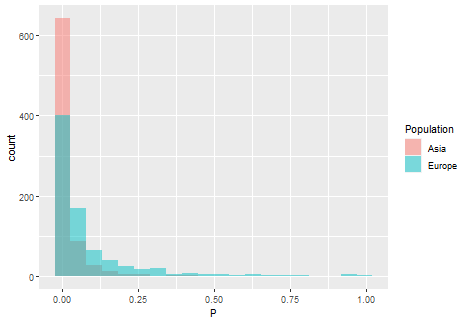
\includegraphics{GWAS-Pvalues_files/figure-latex/visualization-1.png}

Based on the figure above, we can conclude that the distribution of p
values in Asian population is stochastically smaller than the
distribution in European population, even if their underlying
\(\beta_G\) are both \(0.3\). Therefore, it shows that the magnitudes of
p-values of different studies are not directly comparable, unless the
generalized linear regression model being used is the ordinary linear
regression model with \(g\) being identity function.

\clearpage

\hypertarget{simulation-with-case-control-design}{%
\section{Simulation with Case-Control
design:}\label{simulation-with-case-control-design}}

In this section, we will demonstrate the same problem will also occur
for studies with Case-Control design, using a new simulation example.

For the new simulation, we will continue to use the two data-generating
models as in section 2. However, instead of using samples randomly
simulated from the population, we are now randomly sampling from cases
and controls in the following way:

\begin{itemize}
\tightlist
\item
  First, use the two true models to generate two \textbf{populations} of
  size 3000 in the same way as in section 2.
\item
  Secondly, among all the cases and controls in each population,
  randomly sample 500 observations from cases and 500 observations from
  controls.
\item
  Finally, for each population, combine all the sampled cases and
  controls to have a sample with size 1000.
\end{itemize}

\begin{Shaded}
\begin{Highlighting}[]
\CommentTok{### Simulated the common Z and G}
\KeywordTok{set.seed}\NormalTok{(}\DecValTok{100}\NormalTok{,}\DataTypeTok{sample.kind =} \StringTok{"Rounding"}\NormalTok{)}
\NormalTok{N <-}\StringTok{ }\DecValTok{5000}
\NormalTok{G <-}\StringTok{ }\KeywordTok{sample}\NormalTok{(}\KeywordTok{c}\NormalTok{(}\DecValTok{0}\NormalTok{,}\DecValTok{1}\NormalTok{,}\DecValTok{2}\NormalTok{),}\DataTypeTok{size =}\NormalTok{ N, }\DataTypeTok{replace =}\NormalTok{ T, }\DataTypeTok{prob =} \KeywordTok{c}\NormalTok{(}\FloatTok{0.49}\NormalTok{,}\FloatTok{0.42}\NormalTok{,}\FloatTok{0.09}\NormalTok{))}
\NormalTok{Z <-}\StringTok{ }\KeywordTok{rnorm}\NormalTok{(N,}\DataTypeTok{sd =} \DecValTok{3}\NormalTok{)}
\CommentTok{## Eur:}
\NormalTok{beta0 <-}\StringTok{ }\FloatTok{-0.5}
\NormalTok{betaZ <-}\StringTok{ }\FloatTok{0.8}
\NormalTok{betaG <-}\StringTok{ }\FloatTok{0.3}
\NormalTok{ylat_Eur <-}\StringTok{ }\NormalTok{beta0 }\OperatorTok{+}\StringTok{ }\NormalTok{betaG}\OperatorTok{*}\NormalTok{G }\OperatorTok{+}\StringTok{ }\NormalTok{betaZ}\OperatorTok{*}\NormalTok{Z }\OperatorTok{+}\StringTok{ }\KeywordTok{rlogis}\NormalTok{(N)}
\NormalTok{y_Eur <-}\StringTok{ }\KeywordTok{ifelse}\NormalTok{(ylat_Eur }\OperatorTok{>=}\StringTok{ }\DecValTok{0}\NormalTok{, }\DecValTok{1}\NormalTok{, }\DecValTok{0}\NormalTok{)}
\NormalTok{Eur_controls <-}\StringTok{ }\KeywordTok{tibble}\NormalTok{(}\DataTypeTok{Y =}\NormalTok{ y_Eur, }\DataTypeTok{G =}\NormalTok{ G, }\DataTypeTok{Z =}\NormalTok{ Z) }\OperatorTok\StringTok{ }\KeywordTok{filter}\NormalTok{(Y }\OperatorTok{==}\StringTok{ }\DecValTok{0}\NormalTok{) }\OperatorTok\StringTok{ }\KeywordTok{sample_n}\NormalTok{(}\DecValTok{500}\NormalTok{)}
\NormalTok{Eur_cases <-}\StringTok{ }\KeywordTok{tibble}\NormalTok{(}\DataTypeTok{Y =}\NormalTok{ y_Eur, }\DataTypeTok{G =}\NormalTok{ G, }\DataTypeTok{Z =}\NormalTok{ Z) }\OperatorTok\StringTok{ }\KeywordTok{filter}\NormalTok{(Y }\OperatorTok{==}\StringTok{ }\DecValTok{1}\NormalTok{) }\OperatorTok\StringTok{ }\KeywordTok{sample_n}\NormalTok{(}\DecValTok{500}\NormalTok{)}
\NormalTok{EU_sample <-}\StringTok{ }\KeywordTok{rbind}\NormalTok{(Eur_cases,Eur_controls)}
\NormalTok{mod_Eur <-}\StringTok{ }\KeywordTok{glm}\NormalTok{(Y }\OperatorTok{~}\StringTok{ }\NormalTok{Z }\OperatorTok{+}\StringTok{ }\NormalTok{G,}\DataTypeTok{data =}\NormalTok{ EU_sample, }\DataTypeTok{family =} \KeywordTok{binomial}\NormalTok{(}\DataTypeTok{link =} \StringTok{"logit"}\NormalTok{))}
\KeywordTok{summary}\NormalTok{(mod_Eur)}\OperatorTok{$}\NormalTok{coefficients[}\DecValTok{3}\NormalTok{,}\DecValTok{4}\NormalTok{]}
\end{Highlighting}
\end{Shaded}

\begin{verbatim}
## [1] 0.0001973326
\end{verbatim}

\begin{Shaded}
\begin{Highlighting}[]
\CommentTok{## Asia:}
\KeywordTok{set.seed}\NormalTok{(}\DecValTok{100}\NormalTok{,}\DataTypeTok{sample.kind =} \StringTok{"Rounding"}\NormalTok{)}
\NormalTok{beta0 <-}\StringTok{ }\FloatTok{-0.5}
\NormalTok{betaZ <-}\StringTok{ }\FloatTok{0.1}
\NormalTok{betaG <-}\StringTok{ }\FloatTok{0.3}
\NormalTok{ylat_As <-}\StringTok{ }\NormalTok{beta0 }\OperatorTok{+}\StringTok{ }\NormalTok{betaG}\OperatorTok{*}\NormalTok{G }\OperatorTok{+}\StringTok{ }\NormalTok{betaZ}\OperatorTok{*}\NormalTok{Z }\OperatorTok{+}\StringTok{ }\KeywordTok{rlogis}\NormalTok{(N)}
\NormalTok{y_As <-}\StringTok{ }\KeywordTok{ifelse}\NormalTok{(ylat_As }\OperatorTok{>=}\StringTok{ }\DecValTok{0}\NormalTok{, }\DecValTok{1}\NormalTok{, }\DecValTok{0}\NormalTok{)}
\NormalTok{As_controls <-}\StringTok{ }\KeywordTok{tibble}\NormalTok{(}\DataTypeTok{Y =}\NormalTok{ y_As, }\DataTypeTok{G =}\NormalTok{ G, }\DataTypeTok{Z =}\NormalTok{ Z) }\OperatorTok\StringTok{ }\KeywordTok{filter}\NormalTok{(Y }\OperatorTok{==}\StringTok{ }\DecValTok{0}\NormalTok{) }\OperatorTok\StringTok{ }\KeywordTok{sample_n}\NormalTok{(}\DecValTok{500}\NormalTok{)}
\NormalTok{As_cases <-}\StringTok{ }\KeywordTok{tibble}\NormalTok{(}\DataTypeTok{Y =}\NormalTok{ y_As, }\DataTypeTok{G =}\NormalTok{ G, }\DataTypeTok{Z =}\NormalTok{ Z) }\OperatorTok\StringTok{ }\KeywordTok{filter}\NormalTok{(Y }\OperatorTok{==}\StringTok{ }\DecValTok{1}\NormalTok{) }\OperatorTok\StringTok{ }\KeywordTok{sample_n}\NormalTok{(}\DecValTok{500}\NormalTok{)}
\NormalTok{As_sample <-}\StringTok{ }\KeywordTok{rbind}\NormalTok{(As_cases,As_controls)}
\NormalTok{mod_As <-}\StringTok{ }\KeywordTok{glm}\NormalTok{(Y }\OperatorTok{~}\StringTok{ }\NormalTok{Z }\OperatorTok{+}\StringTok{ }\NormalTok{G,}\DataTypeTok{data =}\NormalTok{ As_sample, }\DataTypeTok{family =} \KeywordTok{binomial}\NormalTok{(}\DataTypeTok{link =} \StringTok{"logit"}\NormalTok{))}
\KeywordTok{summary}\NormalTok{(mod_As)}\OperatorTok{$}\NormalTok{coefficients[}\DecValTok{3}\NormalTok{,}\DecValTok{4}\NormalTok{]}
\end{Highlighting}
\end{Shaded}

\begin{verbatim}
## [1] 3.561277e-33
\end{verbatim}

Using Wald test as before, we have p-value (\(5.679 \times 10 ^{-26}\))
in Asian population being much less than the p-value in European
population (\(7.489 \times 10^{-3}\)). Note that we are still assuming
the same \(\tilde{\beta}_G\) for each population in this example.

For case-control data, we cannot directly compute the theoretical power
using the formula from section 1. When a logistic regression model is
fitted for case-control data, the estimated intercept parameter
\(\hat{\beta_0}\) will no longer have the same interpretation as the
\(\beta_0\) we used in the generating model. This implies that we cannot
plug in \(\tilde{\beta}_0=-0.5\) as the true value for the intercept
when we compute theoretical powers. However, we can still obtain the
empirical powers and distribution of p-values using the same approach as
before:

\begin{Shaded}
\begin{Highlighting}[]
\CommentTok{### Simulate each population's disease status based on Z and G}
\CommentTok{## Eur:}
\KeywordTok{set.seed}\NormalTok{(}\DecValTok{100}\NormalTok{,}\DataTypeTok{sample.kind =} \StringTok{"Rounding"}\NormalTok{)}
\NormalTok{beta0 <-}\StringTok{ }\FloatTok{-0.5}
\NormalTok{betaZ <-}\StringTok{ }\FloatTok{0.8}
\NormalTok{betaG <-}\StringTok{ }\FloatTok{0.3}
\NormalTok{p1 <-}\StringTok{ }\KeywordTok{c}\NormalTok{()}
\ControlFlowTok{for}\NormalTok{ (i }\ControlFlowTok{in} \DecValTok{1}\OperatorTok{:}\DecValTok{800}\NormalTok{) \{}
\NormalTok{  ylat_Eur <-}\StringTok{ }\NormalTok{beta0 }\OperatorTok{+}\StringTok{ }\NormalTok{betaG}\OperatorTok{*}\NormalTok{G }\OperatorTok{+}\StringTok{ }\NormalTok{betaZ}\OperatorTok{*}\NormalTok{Z }\OperatorTok{+}\StringTok{ }\KeywordTok{rlogis}\NormalTok{(N)}
\NormalTok{  y_Eur <-}\StringTok{ }\KeywordTok{ifelse}\NormalTok{(ylat_Eur }\OperatorTok{>=}\DecValTok{0}\NormalTok{, }\DecValTok{1}\NormalTok{, }\DecValTok{0}\NormalTok{)}
\NormalTok{  Eur_controls <-}\StringTok{ }\KeywordTok{tibble}\NormalTok{(}\DataTypeTok{Y =}\NormalTok{ y_Eur, }\DataTypeTok{G =}\NormalTok{ G, }\DataTypeTok{Z =}\NormalTok{ Z) }\OperatorTok\StringTok{ }\KeywordTok{filter}\NormalTok{(Y }\OperatorTok{==}\StringTok{ }\DecValTok{0}\NormalTok{) }\OperatorTok\StringTok{ }\KeywordTok{sample_n}\NormalTok{(}\DecValTok{500}\NormalTok{)}
\NormalTok{  Eur_cases <-}\StringTok{ }\KeywordTok{tibble}\NormalTok{(}\DataTypeTok{Y =}\NormalTok{ y_Eur, }\DataTypeTok{G =}\NormalTok{ G, }\DataTypeTok{Z =}\NormalTok{ Z) }\OperatorTok\StringTok{ }\KeywordTok{filter}\NormalTok{(Y }\OperatorTok{==}\StringTok{ }\DecValTok{1}\NormalTok{) }\OperatorTok\StringTok{ }\KeywordTok{sample_n}\NormalTok{(}\DecValTok{500}\NormalTok{)}
\NormalTok{  EU_sample <-}\StringTok{ }\KeywordTok{rbind}\NormalTok{(Eur_cases,Eur_controls)}
\NormalTok{  mod_Eur <-}\StringTok{ }\KeywordTok{glm}\NormalTok{(Y}\OperatorTok{~}\NormalTok{Z }\OperatorTok{+}\StringTok{ }\NormalTok{G,}\DataTypeTok{data =}\NormalTok{ EU_sample, }\DataTypeTok{family =} \KeywordTok{binomial}\NormalTok{(}\DataTypeTok{link =} \StringTok{"logit"}\NormalTok{))}
\NormalTok{  p1[i] <-}\StringTok{ }\KeywordTok{summary}\NormalTok{(mod_Eur)}\OperatorTok{$}\NormalTok{coefficients[}\DecValTok{3}\NormalTok{,}\DecValTok{4}\NormalTok{]}
\NormalTok{\}}
\NormalTok{emp_power <-}\StringTok{ }\KeywordTok{mean}\NormalTok{(p1 }\OperatorTok{<=}\StringTok{ }\NormalTok{alpha)}
\NormalTok{emp_power}
\end{Highlighting}
\end{Shaded}

\begin{verbatim}
## [1] 0.62125
\end{verbatim}

\begin{Shaded}
\begin{Highlighting}[]
\CommentTok{## Asia:}
\KeywordTok{set.seed}\NormalTok{(}\DecValTok{100}\NormalTok{,}\DataTypeTok{sample.kind =} \StringTok{"Rounding"}\NormalTok{)}
\NormalTok{beta0 <-}\StringTok{ }\FloatTok{-0.5}
\NormalTok{betaZ <-}\StringTok{ }\FloatTok{0.1}
\NormalTok{betaG <-}\StringTok{ }\FloatTok{0.3}
\NormalTok{p2 <-}\StringTok{ }\KeywordTok{c}\NormalTok{()}
\ControlFlowTok{for}\NormalTok{ (i }\ControlFlowTok{in} \DecValTok{1}\OperatorTok{:}\DecValTok{800}\NormalTok{) \{}
\NormalTok{  ylat_As <-}\StringTok{ }\NormalTok{beta0 }\OperatorTok{+}\StringTok{ }\NormalTok{betaG}\OperatorTok{*}\NormalTok{G }\OperatorTok{+}\StringTok{ }\NormalTok{betaZ}\OperatorTok{*}\NormalTok{Z }\OperatorTok{+}\StringTok{ }\KeywordTok{rlogis}\NormalTok{(N)}
\NormalTok{  y_As <-}\StringTok{ }\KeywordTok{ifelse}\NormalTok{(ylat_As }\OperatorTok{>=}\DecValTok{0}\NormalTok{, }\DecValTok{1}\NormalTok{, }\DecValTok{0}\NormalTok{)}
\NormalTok{  As_controls <-}\StringTok{ }\KeywordTok{tibble}\NormalTok{(}\DataTypeTok{Y =}\NormalTok{ y_As, }\DataTypeTok{G =}\NormalTok{ G, }\DataTypeTok{Z =}\NormalTok{ Z) }\OperatorTok\StringTok{ }\KeywordTok{filter}\NormalTok{(Y }\OperatorTok{==}\StringTok{ }\DecValTok{0}\NormalTok{) }\OperatorTok\StringTok{ }\KeywordTok{sample_n}\NormalTok{(}\DecValTok{500}\NormalTok{)}
\NormalTok{  As_cases <-}\StringTok{ }\KeywordTok{tibble}\NormalTok{(}\DataTypeTok{Y =}\NormalTok{ y_As, }\DataTypeTok{G =}\NormalTok{ G, }\DataTypeTok{Z =}\NormalTok{ Z) }\OperatorTok\StringTok{ }\KeywordTok{filter}\NormalTok{(Y }\OperatorTok{==}\StringTok{ }\DecValTok{1}\NormalTok{) }\OperatorTok\StringTok{ }\KeywordTok{sample_n}\NormalTok{(}\DecValTok{500}\NormalTok{)}
\NormalTok{  As_sample <-}\StringTok{ }\KeywordTok{rbind}\NormalTok{(As_cases,As_controls)}
\NormalTok{  mod_As <-}\StringTok{ }\KeywordTok{glm}\NormalTok{(Y}\OperatorTok{~}\NormalTok{Z }\OperatorTok{+}\StringTok{ }\NormalTok{G,}\DataTypeTok{data =}\NormalTok{ As_sample, }\DataTypeTok{family =} \KeywordTok{binomial}\NormalTok{(}\DataTypeTok{link =} \StringTok{"logit"}\NormalTok{))}
\NormalTok{  p2[i] <-}\StringTok{ }\KeywordTok{summary}\NormalTok{(mod_As)}\OperatorTok{$}\NormalTok{coefficients[}\DecValTok{3}\NormalTok{,}\DecValTok{4}\NormalTok{]}
\NormalTok{\}}
\NormalTok{emp_power <-}\StringTok{ }\KeywordTok{mean}\NormalTok{(p2 }\OperatorTok{<=}\StringTok{ }\NormalTok{alpha)}
\NormalTok{emp_power}
\end{Highlighting}
\end{Shaded}

\begin{verbatim}
## [1] 0.865
\end{verbatim}

Again, as we have observed in section 2, the empirical powers of Wald
test still differ a lot when we use case-control design (\(0.621\) in
Europe and \(0.865\) in Asia). We can also see the distribution of
p-values for each population:

\begin{Shaded}
\begin{Highlighting}[]
\NormalTok{pcomp <-}\StringTok{ }\KeywordTok{tibble}\NormalTok{(}\DataTypeTok{P =} \KeywordTok{c}\NormalTok{(p1,p2), }\DataTypeTok{Population =} \KeywordTok{c}\NormalTok{(}\KeywordTok{rep}\NormalTok{(}\StringTok{"Europe"}\NormalTok{,}\DecValTok{800}\NormalTok{),}\KeywordTok{rep}\NormalTok{(}\StringTok{"Asia"}\NormalTok{,}\DecValTok{800}\NormalTok{)))}
\NormalTok{pcomp }\OperatorTok\StringTok{ }\KeywordTok{ggplot}\NormalTok{(}\KeywordTok{aes}\NormalTok{(}\DataTypeTok{x =}\NormalTok{ P, }\DataTypeTok{fill =}\NormalTok{ Population)) }\OperatorTok{+}\StringTok{ }\KeywordTok{geom_histogram}\NormalTok{(}\DataTypeTok{bins =} \DecValTok{20}\NormalTok{, }\DataTypeTok{alpha=}\FloatTok{0.5}\NormalTok{, }\DataTypeTok{position=}\StringTok{"identity"}\NormalTok{)}
\end{Highlighting}
\end{Shaded}

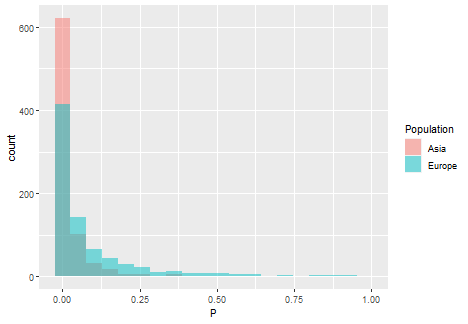
\includegraphics{GWAS-Pvalues_files/figure-latex/visualCaseControl-1.png}
As we can see, the conclusion from section 2 still applies to this
scenario. The rationale behind these two simulation examples is that,
statistical significance (i.e.~P value) does not give any information on
the \textbf{practical significance} (i.e.~\(|\tilde{\beta}_G|\)). For
both populations, the practical significance of parameter \(\beta_G\) is
the same (0.3). However, testing in the Asian population gives higher
statistical significance (smaller p values), due to the larger standard
error caused by the higher \(\beta_Z\).

Therefore, screening out SNPs based on the significance from study in
the European population might miss this casual SNP, but screening based
on the Asian population likely will not. Extra caution should be given
when practitioners are trying to aggregate information between two such
populations.

\hypertarget{bibliography}{%
\section{Bibliography}\label{bibliography}}

\setlength{\parindent}{-0.2in}
\setlength{\leftskip}{0.2in}
\setlength{\parskip}{8pt}

\noindent

\hypertarget{refs}{}
\leavevmode\hypertarget{ref-meta1}{}%
Begum, Ferdouse, Debashis Ghosh, George C. Tseng, and Eleanor Feingold.
2012. ``Comprehensive literature review and statistical considerations
for GWAS meta-analysis.'' \emph{Nucleic Acids Research} 40 (9):
3777--84. \url{https://doi.org/10.1093/nar/gkr1255}.

\leavevmode\hypertarget{ref-meta2}{}%
Evangelou, Evangelos, and John Ioannidis. 2013. ``Evangelou E, Ioannidis
Jp.meta-Analysis Methods for Genome-Wide Association Studies and Beyond.
Nat Rev Genet 14:379-389.'' \emph{Nature Reviews. Genetics} 14 (May).
\url{https://doi.org/10.1038/nrg3472}.

\end{document}
